\documentclass[english,letter paper,12pt,reqno]{article}
\usepackage{etex} % to fix "no room for new dimen" error. Voodoo.
\usepackage{array}
\usepackage{bussproofs}
\usepackage{stmaryrd}
\usepackage{amsmath, amscd, amssymb, mathrsfs, accents, amsfonts,amsthm}
\usepackage[all]{xy}
\usepackage{mathtools} % for bra-ket
\usepackage{tikz}
\usetikzlibrary{calc}

\AtEndDocument{\bigskip{\footnotesize%
  \textsc{Department of Mathematics, University of Southern California} \par  
  \textit{E-mail address}: \texttt{murfet@usc.edu} \par
}}

% Labels in tabular
\newcommand{\tagarray}{\mbox{}\refstepcounter{equation}$(\theequation)$}

% Bra-ket stuff
\DeclarePairedDelimiter\bra{\langle}{\rvert}
\DeclarePairedDelimiter\ket{\lvert}{\rangle}
\DeclarePairedDelimiterX\braket[2]{\langle}{\rangle}{#1 \delimsize\vert #2}
\DeclarePairedDelimiterX\inner[2]{\langle}{\rangle}{#1,#2}
\DeclarePairedDelimiter\abs{\lvert}{\rvert}
\DeclarePairedDelimiter\norm{\lVert}{\rVert}
\DeclarePairedDelimiter\set{\lbrace}{\rbrace}

%\begin{align*}
%\bra{a}       &= \bra*{\frac{a}{1}}\    \ket{a}       &= \ket*{\frac{a}{1}}\    \braket{a}{b} &= \braket*{\frac{a}{1}}{\frac{b}{1}}\    %\inner{a}{b}  &= \inner*{\frac{a}{1}}{\frac{b}{1}}\    \abs{a}       &= \abs*{\frac{a}{1}}\    \norm{a}      &= \norm*{\frac{a}%{1}}\    \set{a,b}     &= \set*{\frac{a}{1},\frac{b}{1}}
%\end{align*}

% TikZ stuff
\def\drawbang{\draw[color=teal!50, line width=2pt]}
\def\drawprom{\draw[color=gray, line width=3pt]}
\def\bluenode{\node[circle,draw=blue!50,fill=blue!20]}
\def\mapnode{\node[circle,draw=black,fill=black,inner sep=0.5mm]}
\def\whitenode{\node[circle,draw=blue!50,fill=blue!5]}
\def\dernode{\node[circle,draw=black,fill=white]}
\definecolor{Myblue}{rgb}{0,0,0.6}
\usepackage[a4paper,colorlinks,citecolor=Myblue,linkcolor=Myblue,urlcolor=Myblue,pdfpagemode=None]{hyperref}

\SelectTips{cm}{}

\setlength{\evensidemargin}{0.1in}
\setlength{\oddsidemargin}{0.1in}
\setlength{\textwidth}{6.3in}
\setlength{\topmargin}{0.0in}
\setlength{\textheight}{8.5in}
\setlength{\headheight}{0in}

\newtheorem{theorem}{Theorem}[section]
\newtheorem{proposition}[theorem]{Proposition}
\newtheorem{lemma}[theorem]{Lemma}
\newtheorem{corollary}[theorem]{Corollary}

\newtheoremstyle{example}{\topsep}{\topsep}
	{}
	{}
	{\bfseries}
	{.}
	{2pt}
	{\thmname{#1}\thmnumber{ #2}\thmnote{ #3}}
	
	\theoremstyle{example}
	\newtheorem{definition}[theorem]{Definition}
	\newtheorem{example}[theorem]{Example}
	\newtheorem{remark}[theorem]{Remark}
	\newtheorem{question}[theorem]{Question}

\numberwithin{equation}{section}

% Operators
\def\eval{\operatorname{ev}}
\def\sh{\operatorname{Sh}}
\def\res{\operatorname{Res}}
\def\Coker{\operatorname{Coker}}
\def\Ker{\operatorname{Ker}}
\def\im{\operatorname{Im}}
\def\can{\operatorname{can}}
\def\K{\mathbf{K}}
\def\D{\mathbf{D}}
\def\N{\mathbf{N}}
\def\LG{\mathcal{LG}}
\def\Ab{\operatorname{Ab}}
\def\Hom{\operatorname{Hom}}
\def\modd{\operatorname{mod}}
\def\Modd{\operatorname{Mod}}
\DeclareMathOperator{\Ext}{Ext}
\DeclareMathOperator{\Tr}{Tr}
\DeclareMathOperator{\End}{End}
\DeclareMathOperator{\rank}{rank}
\DeclareMathOperator{\tot}{Tot}
\DeclareMathOperator{\ch}{ch}
\DeclareMathOperator{\str}{str}
\DeclareMathOperator{\hmf}{hmf}
\DeclareMathOperator{\HMF}{HMF}
\DeclareMathOperator{\hf}{HF}
\DeclareMathOperator{\At}{At}
\DeclareMathOperator{\Cat}{Cat}
\DeclareMathOperator{\Spec}{Spec}
\DeclareMathOperator{\MSpec}{MSpec}
\DeclareMathOperator{\Sym}{Sym}
\DeclareMathOperator{\LC}{LC}
\def\inta{\bold{int}}
\def\contract{\;\lrcorner\;}

% SCprooftree environment
\newenvironment{scprooftree}[1]
{\gdef\scalefactor{#1}\begin{center}\proofSkipAmount \leavevmode}
{\scalebox{\scalefactor}{\DisplayProof}\proofSkipAmount \end{center} }
  
\begin{document}

% Bussproof things
\def\ScoreOverhang{1pt}

% Commands
\def\Res{\res\!}
\newcommand{\ud}[1]{\operatorname{d}\!{#1}}
\newcommand{\Ress}[1]{\res_{#1}\!}
\newcommand{\cat}[1]{\mathcal{#1}}
\newcommand{\lto}{\longrightarrow}
\newcommand{\xlto}[1]{\stackrel{#1}\lto}
\newcommand{\mf}[1]{\mathfrak{#1}}
\newcommand{\md}[1]{\mathscr{#1}}
\newcommand{\church}[1]{\underline{#1}}
\newcommand{\prf}[1]{\underline{#1}}
\newcommand{\den}[1]{\llbracket #1 \rrbracket}
\def\l{\,|\,}
\def\sgn{\textup{sgn}}
\def\cont{\operatorname{cont}}

\title{Logic and linear algebra: geometry of interaction}
\author{Daniel Murfet}

\maketitle

Girard's original geometry of interaction model \cite{girard_goi1} works as follows: if $\mathbb{H}$ is the Hilbert space of square-summable sequences in $\mathbb{C}$ then he assigns to each proof (in full linear logic) of a sequent $\vdash A_1,\ldots,A_n$ with cuts on formulas $B_1,\ldots,B_m$ a bounded linear operator on $\mathbb{H}^{2m+n}$. Tracing out the $2m$ factors of $\mathbb{H}$ yields an operator on $\mathbb{H}^n$ which agrees with the operator assigned to the cut-free normalisation of the original proof. This operation of ``tracing out the cuts'' is the dynamics which models the process of cut-elimination; it can be rephrased as a sum over paths in a graph associated to the proof \cite{danos_regnier2}.

A simplified example using the vector space semantics can capture the key idea. Let us suppose in the above that $\den{B}$ is a finite-dimensional vector space. Then $\den{\rho} \circ \den{\pi}$ may be computed as a trace
\begin{equation}
\den{\rho} \circ \den{\pi} = \operatorname{tr}_{\den{B}}\big( \sigma \circ (\den{\pi} \otimes \den{\rho}) \big)
\end{equation}
where $\sigma: \den{B} \otimes \den{C} \lto \den{C} \otimes \den{B}$ is the symmetry map and $\operatorname{tr}_{\den{B}}$ is a partial trace. Using the standard notation for traces in string diagrams \cite{joyal_trace} this reads:
\begin{center}
\begin{tabular}{>{\centering}m{2cm} >{\centering}m{1cm} m{4cm}}
\begin{tikzpicture}[inner sep = 0.5mm, scale=0.4,auto]
\node (bottom) at (0,-5) {$A$};
\node (top) at (0,5) {$C$};
\node[circle,draw=black,fill=black] (o) at (0,2) {};
\node [above] at (o.east) {$\;\;\;\;\;\;\den{\rho}$};
\node[circle,draw=black,fill=black] (o) at (0,-2) {};
\node [above] at (o.east) {$\;\;\;\;\;\;\den{\pi}$};
\draw (bottom) to (o);
\draw (o) to (top);
\end{tikzpicture}
& = &
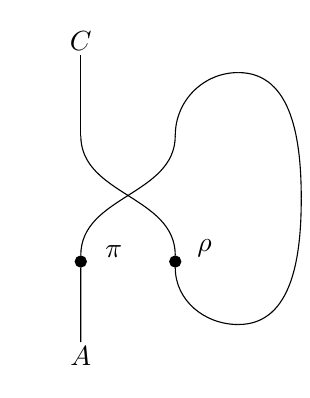
\begin{tikzpicture}[inner sep = 0.5mm, scale=0.4,auto]
\node (bottom) at (-1,-5) {$A$};
\node (top) at (-1,5) {$C$};
\node[circle,draw=black,fill=black] (o) at (-1,-2) {};
\node [above] at (o.east) {$\;\;\;\;\;\;\;\den{\pi}$};
\node[circle,draw=black,fill=black] (q) at (2,-2) {};
\node [above] at (q.east) {$\;\;\;\;\;\;\den{\rho}$};
\coordinate (turn_bottom) at (4,-4);
\coordinate (turn_top) at (4,4);
\coordinate (right) at (6,0);
\coordinate (base_top) at (2,2);
\coordinate (other_top) at (-1,2);
\draw (bottom) to (o);
\draw[out=270,in=180] (q) to (turn_bottom);
\draw[out=0,in=270] (turn_bottom) to (right);
\draw[out=90,in=0] (right) to (turn_top);
\draw[out=180,in=90] (turn_top) to (base_top);
\draw[out=270,in=90] (base_top) to (o);
\draw[out=90,in=270] (q) to (other_top);
\draw (other_top) to (top);
\end{tikzpicture}
\end{tabular}
\end{center}
The upshot is that we may view the tensor $\den{\pi} \otimes \den{\rho}$ together with the information of the tensor factor $\den{B}$ as an intermediate step between $\den{\pi}$ and the composite $\den{\rho} \circ \den{\pi}$. That is, the two syntactical steps of \eqref{eq:cut_elim_step} correspond to the sequence
\[
\den{\pi} \longmapsto \big( \den{\pi} \otimes \den{\rho}, \den{B} \big) \longmapsto \operatorname{tr}_{\den{B}}\big( \sigma \circ  (\den{\pi} \otimes \den{\rho})\big) = \den{\rho} \circ \den{\pi}\,.
\]
Since traces are only available for finite-dimensional spaces this idea cannot be extended to arbitrary $\den{B}$ and is therefore not to be taken seriously, but there are numerous traced monoidal categories where a similar construction can be formalised \cite{abramsky3,abramsky4,abramsky2}. In particular, Girard's original model using Hilbert spaces can be formulated in these terms; see the introductory notes by Shirahata \cite{shirahata} and Haghverdi-Scott \cite{haghverdi}.
\\

Next we consider examples of ``explicitation'' in geometry, which leads to a discussion of semantics of cut-elimination in bicategories of geometric spaces and the ideas behind \cite{murfet}. In modern geometry we often understand spaces via the vector bundles living on them, and these we in turn understand via their characteristic classes, which are elements in finite-dimensional vector spaces called cohomology groups. However, \emph{implicit} knowledge of a vector in some cohomology group, say produced from a series of abstract maps, should be distinguished from \emph{explicit} knowledge, say coefficients in a preferred basis.

The prototypical example is Hodge theory. Let $M$ be an $n$-dimensional compact oriented smooth manifold. The de Rham cohomology of $M$ \cite{bott} is the cohomology of the complex of global sections of the sheaf of differential forms
\[
\xymatrix{
0 \ar[r] & \Omega^0(M) \ar[r]^-{d^0} & \cdots \ar[r] & \Omega^p(M) \ar[r]^-{d^p} & \Omega^{p+1}(M) \ar[r] & \cdots \ar[r] & \Omega^n(M) \ar[r] & 0
}\,.
\]
If $Z^p(M) = \Ker(d^p)$ denotes the closed $p$-forms and $B^p(M) = \im(d^{p-1})$ the exact $p$-forms, then the $p$th de Rham cohomology group is
\[
H^p(M) = \frac{Z^p(M)}{B^p(M)}\,.
\]
By a theorem of Hodge a preferred basis is given for each $p$ by the subspace of harmonic forms $\mathscr{H}^p(M) \subseteq Z^p(M)$. That is, there is an isomorphism
\[
\xymatrix{
\mathscr{H}^p(M) \ar[r] & Z^p(M) \ar[r] & Z^p(M)/B^p(M) = H^p(M)
}\,.
\]
Giving an equivalence class of vectors in $Z^p(M)$ is therefore equivalent to specifying an element in $\mathscr{H}^p(M)$, but since $Z^p(M)$ is infinite-dimensional these two forms of knowledge have a different character. For example, exhibiting the coefficients of the equivalence class of a vector $\eta \in Z^p(M)$ in a chosen basis $\{ \omega_i \}_i$ of harmonic forms requires additional work, which takes the form of computing integrals:
\begin{equation}\label{eq:basis_harmonic}
\eta \equiv \sum_i \langle \eta, \omega_i \rangle \omega_i, \qquad \langle \eta, \omega_i \rangle = \int_M \eta \wedge \star\, \omega_i\,.
\end{equation}
To connect this back to computation and the sequence \eqref{eq:cut_elim_step}, let $M,N$ be smooth projective varieties over $\mathbb{C}$. Any cohomology class $\rho \in H^*(M \times N)$ determines a linear map of finite-dimensional vector spaces
\begin{gather*}
I_\rho: H^*(M) \lto H^*(N)\,,\\
\pi \longmapsto (p_N)_*( \rho \cup p_M^*(\pi) )
\end{gather*}
where $p_M, p_N$ denote the projections from $M \times N$. Suppose that we insist on dealing only with harmonic forms. Then to compute $I_\rho$ on some ``input'' harmonic form $\pi$ and get a harmonic form as ``output'' we apply the following composite
\begin{gather*}
\xymatrix{
\mathscr{H}^*(M) \ar[r]^-{\cong} & H^*(M) \ar[r]^-{I_\rho} & H^*(N) \ar[r]^-{\cong} & \mathscr{H}^*(N)
}\\
\pi \longmapsto I_\rho(\pi) \longmapsto \sum_j \langle I_\rho(\pi), \omega_j \rangle \omega_j\,.
\end{gather*}
A comparision of this process -- first compute $I_\rho$ and then project onto harmonic forms using the integrals in \eqref{eq:basis_harmonic} -- with the two syntactical steps of \eqref{eq:cut_elim_step} suggests a natural starting point for a search for semantics of cut-elimination in geometry, with integration playing the role of explicitation.
\\

However, given the expectation previously expressed of higher-categorical semantics of cut-elimination, it is natural to start the search not with cohomology and linear maps but categories and functors. In this setting the relationship between the space of harmonic forms $\mathscr{H}^*(M)$ and the de Rham cohomology $H^*(M)$ may be compared to that between the bounded derived category of coherent sheaves $\mathbf{D}^b(\operatorname{coh} M)$ and the full subcategory $\mathbf{D}^b_{\operatorname{coh}}(\operatorname{Qco} M)$ of complexes with bounded, coherent cohomology in the unbounded derived category of quasi-coherent sheaves $\mathbf{D}(\operatorname{Qco} M)$.\footnote{We do not intend to compare harmonic forms with arbitrary complexes of coherent sheaves. The point of the analogy is that $\mathscr{H}^*(M)$ provides an explicit finite-dimensional model for de Rham cohomology. The precise nature of the classes that make up this model is of secondary importance.} These are equivalent categories
\begin{equation}\label{eq:equiv_point}
\xymatrix{
\mathbf{D}^b(\operatorname{coh} M) \ar[r]^-{\cong} & \mathbf{D}^b_{\operatorname{coh}}(\operatorname{Qco} M) \subset \mathbf{D}(\operatorname{Qco} M)
}
\end{equation}
which means that for any object $\md{G}$ of $\mathbf{D}^b_{\operatorname{coh}}(\operatorname{Qco} M)$ there exists an isomorphic bounded complex of coherent sheaves $\md{G}_{\operatorname{finite}}$ which we call a \emph{finite model} of $\md{G}$. But given $\md{G}$ it is not obvious how to produce this finite model in any reasonably algorithmic way.\footnote{Unfortunately this is not a very precise statement, since it depends what we mean by ``reasonable''. While we can reconstruct a complex up to quasi-isomorphism from truncations and in this way construct an explicit complex of coherent sheaves, this is not an algorithm of the kind that we want -- consider the enormous complexity of the complexes produced by taking global sections of an explicit resolution of a sheaf $\md{F}$ by injective quasi-coherent sheaves on a non-trivial scheme. In principle the data in this resolution is determined by $\md{F}$, but it would be madness to build a model of computation on top of objects that are so difficult to handle.} Consider that in the special case where $M$ is a point, \eqref{eq:equiv_point} is an equivalence
\[
\xymatrix{
\mathbf{D}^b(\operatorname{vect} \mathbb{C}) \ar[r]^-{\cong} & \mathbf{D}^b_{\operatorname{fd}}(\operatorname{Vect} \mathbb{C}) \subset \mathbf{D}(\operatorname{Vect} \mathbb{C})
}
\]
between bounded complexes of finite-dimensional vector spaces and unbounded complexes of (infinite-dimensional) vector spaces with finite-dimensional cohomology. For general $M$, if $f: M \lto \mathbb{C}$ denotes the structure map then for a coherent sheaf $\md{F}$ on $M$ the derived pushforward $\mathbb{R} f_*( \md{F} )$ may be defined as an object of $\mathbf{D}^b_{\operatorname{fd}}(\operatorname{Vect} \mathbb{C})$ by a simple universal property, but explicitly computing the isomorphic \emph{finite} complex in $\mathbf{D}^b(\operatorname{vect} \mathbb{C})$ -- that is, computing the cohomology of $\md{F}$ -- requires work to be performed. %, similar to the integrals against harmonic forms in \eqref{eq:basis_harmonic}.

To complete the analogy with the above, suppose we are given a complex of coherent sheaves $\md{R} \in \mathbf{D}^b(\operatorname{coh} M \times N)$, which will play the role of $\rho$. There is a naturally associated triangulated functor
\begin{gather}\label{eq:infinite_functor}
I_{\md{R}}: \mathbf{D}^b_{\operatorname{coh}}(\operatorname{Qco} M) \lto \mathbf{D}^b_{\operatorname{coh}}(\operatorname{Qco} N),\\
\md{F} \longmapsto (p_N)_*( \md{R} \otimes p_M^*( \md{F} ))
\end{gather}
where $p_N: M \times N \lto N$ and $p_M: M \times N \lto M$ are the projections and $(p_N)_*, p^*_M$ denote derived functors. Note that the functor $I_{\md{R}}$ naturally produces infinite complexes of quasi-coherent sheaves with bounded coherent cohomology; rarely will the construction output an actual bounded complex of coherent sheaves. If we want to work with finite objects, computing $I_{\md{R}}$ on some input therefore requires two steps
\begin{gather}\label{eq:step_by_step}
\xymatrix{
\mathbf{D}^b(\operatorname{coh} M) \ar[r]^-{\cong} & \mathbf{D}^b_{\operatorname{coh}}(\operatorname{Qco} M) \ar[r]^-{I_{\md{R}}} & \mathbf{D}^b_{\operatorname{coh}}(\operatorname{Qco} N) \ar[r]^-{\cong} & \mathbf{D}^b(\operatorname{coh} N)
}\\
\md{F} \longmapsto I_{\md{R}}(\md{F}) \longmapsto I_{\md{R}}(\md{F})_{\operatorname{finite}}\,.
\end{gather}
That is, given the input complex $\md{F}$ we first compute $I_{\md{R}}$ and then we take a finite model, which is the form of explicitation natural to algebraic geometry.
\\

This suggests that in a model of computation where proofs or programs are interpreted by functors between triangulated categories, cut-elimination should be interpreted as the algorithmic construction of finite models. But what do we mean when we say that some kind of mathematical structure ``interprets'' cut-elimination? Since categories, functors and natural transformations form a bicategory, our answer is given in terms of bicategorical semantics where types are assigned objects and proofs are assigned $1$-morphisms. 

Taking Girard's geometry of interaction as our guide, we ask for (at least) the following two desiderata. The algorithm computing finite models should be compatible with
\begin{itemize}
\item[(A)] the structure of ambient symmetric monoidal bicategory, and
\item[(B)] the comonad interpretating the exponential modality.
\end{itemize}  
The precise form of these requirements will depend on the bicategory under consideration. In the rest of this section we first sketch the kind of bicategorical semantics of linear logic that we have in mind, and then we explain how the cut systems of \cite{murfet} provide one way of making precise the notion of an ``algorithm for computing finite models''. In the present discussion the two most relevant examples of bicategories are
\begin{itemize}
\item The bicategory $\cat{V}ar$ \cite{ct1007.2679} where objects are smooth projective varieties $M,N,\ldots$ and $1$-morphisms $M \lto N$ are bounded complexes of coherent sheaves 
\[
\cat{V}ar(M,N) = \mathbf{D}^b(\operatorname{coh} M \times N)\,.
\]
For an example of the composition rule, note that if $\md{R} \in \cat{V}ar(M,N)$ and $S$ is a point then composition with $\md{R}$ in this bicategory is a functor $\cat{V}ar(S,M) \lto \cat{V}ar(S,N)$ which is in fact \eqref{eq:infinite_functor}.

\item The bicategory $\LG$ of Landau-Ginzburg models \cite{McNameethesis, lgdual, cr0909.4381} where objects are isolated hypersurface singularities $W,V,\ldots$ and $1$-morphisms $W \lto V$ are finite-rank matrix factorisations of $V - W$
\[
\LG(W,V) = \hmf( V - W )^\omega\,.
\]
Here $\hmf(V - W)$ denotes the homotopy category of matrix factorisations, and $(-)^\omega$ the idempotent completion \cite{Yoshino90}.
\end{itemize}

The bicategories $\cat{V}ar$ and $\LG$ are symmetric monoidal but do not have enough colimits to interpret the exponential modality. However, suitable enlargements of both examples yield bicategories $\cat{C}$ which are symmetric monoidal with an internal Hom and admit a cofree cocommutative coalgebra ${!} V$ for each object $V$. It therefore makes sense to define a semantics of intuitionistic linear logic in $\cat{C}$ (or at least, in the classifying category of $\cat{C}$) where the denotation of a proof is a $1$-morphism. For example, the interpretation of the Church numeral $\church{2}$ is a $1$-morphism
\begin{equation}
\xymatrix@C+0.5pc{
{!} \End(V) \ar[r]^-{\Delta} & {!} \End(V) \otimes {!} \End(V) \ar[r]^-{d \otimes d} & \End(V)^{\otimes 2} \ar[r]^-{- \circ -} & \End(V)
}
\end{equation}
where $\End(V)$ denotes an object of $\cat{C}$ computed using the internal Hom. If we had started with a bicategory of rings and bimodules, this construction would yield the program \eqref{eq:church_as_bimod} from the introduction. 

To explain the interpretation of cut-elimination in such bicategorical semantics we begin by supposing that we have a bicategory $\cat{B}$ and for each pair of objects $M,N$ a full subcategory $\cat{A}(M,N) \subseteq \cat{B}(M,N)$ such that the inclusion is an equivalence. The intuition is that $\cat{A}$ is a collection of ``finite models'' and that every $1$-morphism is isomorphic to some finite model. We do not assume that $\cat{A}$ is a sub-bicategory: the whole point is that the composition in $\cat{B}$ of $1$-morphisms in $\cat{A}$ will not in general belong to $\cat{A}$.

\begin{example} In the case of $\cat{B} = \cat{V}ar$,
\begin{equation}\label{eq:example_bicat}
\cat{A}(M,N) = \mathbf{D}^b(\operatorname{coh} M \times N), \qquad \cat{B}(M,N) = \mathbf{D}^b_{\operatorname{coh}}(\operatorname{Qco} M \times N)\,.
\end{equation}
In the case of $\cat{B} = \LG$ both $W,V$ are the defining equations of singularities and
\begin{equation}\label{eq:example_bicat_hmf}
\cat{A}(W,V) = \hmf( V - W )^\omega, \qquad \cat{B}(W,V) = \HMF_{\operatorname{fd}}( V - W )
\end{equation}
where $\HMF_{\operatorname{fd}}(W)$ denotes the homotopy category of infinite-rank matrix factorisations which are direct summands of finite rank ones. 
\end{example}

The guiding principle is that the denotation in $\cat{B}$ of a cut-free proof should be \emph{finite}, that is, it should be a $1$-morphism in $\cat{A}$. Denotations of proofs with cuts will be defined using the composition operation in $\cat{B}$ and may generate $1$-morphisms outside of $\cat{A}$. The idea is to look for the shadow of the cut-elimination process in $\cat{B}$ in terms of the algorithm which reflects these $1$-morphisms back into $\cat{A}$. We refine this idea into precise mathematics in a series of steps. For any object $S$ the composition in $\cat{B}$ gives a functor
\begin{gather}\label{eq:comp_blahde}
\cat{A}(S,M) \otimes \cat{A}(M,N) \lto \cat{B}(S,N),\\ \qquad \md{F} \otimes \md{R} \mapsto \md{R} \circ \md{F}\,.
\end{gather}
By assumption there is an object $(\md{R} \circ \md{F})_{\operatorname{finite}}$ of $\cat{A}(S,N)$ isomorphic to $\md{R} \circ \md{F}$. Adding this step of taking these finite models to the end of \eqref{eq:comp_blahde} we have
\begin{gather}\label{eq:comp_plus_finite}
\cat{A}(S,M) \otimes \cat{A}(M,N) \lto \cat{B}(S,N) \lto \cat{A}(S,N)\\
\md{F} \otimes \md{R} \longmapsto \md{R} \circ \md{F} \longmapsto (\md{R} \circ \md{F})_{\operatorname{finite}}\,.
\end{gather}
The problem with this construction is that in the examples of interest there is no algorithmic construction of these finite models (of the kind we need) starting from just the data of the object $\md{R} \circ \md{F}$. But what we can do for $\LG$ is refine the composition operation so that it lands not in $\cat{B}(S,N)$ but in an auxiliary category, the Clifford thickening of $\cat{A}(S,N)$, for which an algorithmic construction of objects in $\cat{A}(S,N)$ is under good control.

From now on we assume that $\cat{B}$ is a superbicategory \cite[\S 2.1]{murfet}, which is true of $\LG$ but not of $\cat{V}ar$. In particular the $\cat{A}(M,N)$ are all supercategories. The Clifford thickening of a supercategory is defined using Clifford algebras $A_n$ of dimension $2^{2n}$ with $A_0 = k$. Each of these algebras has a basic representation, the spinor representation $S_n$, such that $A_n = \End_k(S_n)$. This means that every representation $Q$ of $A_n$ in the category of vector spaces is of the form $Q \cong S_n \otimes_k V$ for some $\mathbb{Z}_2$-graded vector space $V$, but the crucial point is that there is some computational ``cost'' associated with extracting the vector space $V$ from $Q$. This may be represented either as computing a tensor product with the dual of the spinor representation $S_n^* = \Hom_k(S_n,k)$
\begin{equation}\label{eq:extract_V}
V \cong S_n^* \otimes_{A_n} Q
\end{equation}
or equivalently as splitting idempotents on $Q$ arising from the Clifford action. When $Q$ is not a vector space but an object of the supercategory $\cat{A}(M,N)$ this extraction process is the form of explicitation which models cut-elimination in a cut-system.

To elaborate, we need to use the \emph{Clifford thickening} $\cat{A}(M,N)^\bullet$ which is the category of all representations of the various Clifford algebras $A_n$ in $\cat{A}(M,N)$. More precisely, an object of this category is object of $\cat{A}(M,N)$ together with the action of a Clifford algebra $A_n$ for some $n \ge 0$. There is an equivalence of supercategories
\begin{equation}\label{eq:land_in_clifford}
\xymatrix{
\cat{A}(M,N) \ar[r]^-{\cong} & \cat{A}(M,N)^\bullet 
}
\end{equation}
which sends an object $\md{F}$ of $\cat{A}(M,N)$ to itself viewed as a representation of $A_0 = k$. The point is that the inverse of this equivalence has a very regular form: given an object $(\md{G}, \zeta)$ of $\cat{A}(M,N)^\bullet$, which is an object $\md{G}$ together with a morphism of algebras
\[
\zeta: A_n \lto \End^*_{\cat{A}(M,N)}( \md{G} )
\]
for some $n$, the tensor product
\begin{equation}\label{eq:extraction_tensor}
\widetilde{\md{G}} := S_n^* \otimes_{A_n} \md{G}
\end{equation}
is an object of $\cat{A}(M,N)$ and the map $(\md{G}, \zeta) \mapsto \widetilde{\md{G}}$ gives an inverse to \eqref{eq:land_in_clifford}. This inverse is analogous to the extraction of the vector space $V$ from the representation $Q$. Note that while $\md{G}$ and $\widetilde{\md{G}}$ are isomorphic objects in the Clifford thickening they represent different states of knowledge: in $\md{G}$ the underlying object of $\cat{A}(M,N)$ is still implicit, while in $\widetilde{\md{G}}$ it has been made explicit. Let us now assume that there is an algorithm for computing the tensor product \eqref{eq:extraction_tensor} so that the inverse to \eqref{eq:land_in_clifford} is under control.\footnote{This algorithm depends on the underlying algebraic objects that make up the bicategory. In the case of $\LG$, computing the tensor product is done by splitting idempotents, which reduces to a computation in commutative algebra using well-understood algorithms.} Thus it only remains to refine the composition in \eqref{eq:comp_blahde} to land in $\cat{A}(S,N)^\bullet$.

That is, we ask for a collection of functors, indexed by triples $M,N,S$
\begin{gather}\label{eq:cut_functors}
\cat{A}(S,M) \otimes \cat{A}(M,N) \lto \cat{A}(S,N)^\bullet\,,\\
\md{F} \otimes \md{R} \longmapsto \md{R} \l \md{F}
\end{gather}
which satisfy some natural axioms. We call $\md{F} \l \md{R}$ the \emph{cut} of $\md{F}$ and $\md{R}$. It is an object of $\cat{A}(S,N)$ together with the action of some Clifford algebra. To say that these cut functors refine the composition operation in $\cat{B}$ is to ask that the following diagram commutes up to natural isomorphism:
\begin{equation}\label{eq:cut_relate}
\xymatrix@C+2pc{
\cat{B}(S,M) \otimes \cat{B}(M,N) \ar[r]^-{- \circ -} & \cat{B}(S,N) & \cat{A}(S,N) \ar[l]_-{\cong} \ar[d]^-{\cong}\\
\cat{A}(S,M) \otimes \cat{A}(M,N) \ar[u]^-{\cong} \ar[rr]_-{- \l -} & & \cat{A}(S,N)^\bullet
}\,.
\end{equation}
Commutativity of this diagram allows us to replace the sequence of steps in \eqref{eq:comp_plus_finite}, that is, the clockwise direction from the bottom left of the diagram \eqref{eq:cut_relate} to the top right
\begin{equation}\label{eq:not_really_cutelim}
\md{F} \otimes \md{R} \longmapsto \md{R} \circ \md{F} \longmapsto (\md{R} \circ \md{F})_{\operatorname{finite}}
\end{equation}
with the series of steps in the anti-clockwise direction
\begin{equation}\label{eq:really_cut_elim}
\md{F} \otimes \md{R} \longmapsto \md{R} \l \md{F} \longmapsto \widetilde{ \md{R} \l \md{F} } := S_n^* \otimes_{A_n} ( \md{R} \l \md{F} )
\end{equation}
The point is that the last step of \eqref{eq:not_really_cutelim} is not under algorithmic control, but every step of \eqref{eq:really_cut_elim} is algorithmic.

In summary the \emph{cut system} $\cat{A}$ which is the collection of categories $\cat{A}(M,N)$ and the cut functors \eqref{eq:cut_functors} gives a precise meaning to the idea of an algorithmic construction of finite models for the result of composition of $1$-morphisms in $\cat{B}$, and this is the structure in the bicategorical semantics which we intend as a model of cut-elimination. The main result of \cite{murfet} is that in the case $\cat{B} = \LG$ there is a natural cut system realising the above. Regarding the desiderata A and B, which must be present before we can call this a model of cut-elimination: while compatibility with the basic structure of the bicategory is part of the axiomatics of a cut system \cite[\S 3]{murfet}, this first paper does not include the compatibility with the tensor product, the internal Hom or finite products. These arguments, together with the verification of desiderata B, will be the subject of future work.

To connect this explicitly back to Girard's ideas in the geometry of interaction, suppose that $\cat{B}$ carries an interpretation of linear logic and that we have a pair of proofs $\pi, \rho$ as in \eqref{goi_prooftree}. Then using the cut system structure we would make the assignments
\begin{align*}
\den{\rho} &= \md{R},\\
\den{\pi} &= \md{F},\\
\den{\rho \l \pi} &= \md{R} \l \md{F},\\
\den{\widetilde{\rho \l \pi}} &= \widetilde{ \md{R} \l \md{F} }\,.
\end{align*}
The ``dynamics'' which generates $\widetilde{ \md{R} \l \md{F} }$ from $\md{R} \l \md{F}$ is the computation of the tensor product with the dual of the spinor representation $S_n^*$ \cite[\S 3.1]{murfet}. 

\begin{example}\label{example:cut_system_hom} The polynomial $0$ is an object of $\cat{B} = \LG$ and with $\cat{A}$ as in \eqref{eq:example_bicat_hmf} for any hypersurface singularity $W$, we have
\begin{align*}
\cat{A}(0, W) &= \hmf(W)^\omega, & \cat{A}(W,0) &= \hmf(-W)^\omega,\\
\cat{A}(0,0) &= \cat{C}_2( k ), & \cat{B}(0,0) &= \cat{C}^\infty_2(k)\,.
\end{align*}
where $\cat{C}_2(k)$ is the homotopy category of $\mathbb{Z}_2$-graded complexes of finite-dimensional $k$-vector spaces and $\cat{C}^\infty_2(k)$ is the homotopy category of infinite-rank complexes with finite-dimensional cohomology. Moreover $\cat{A}(0,0)^\bullet$ is the category of $A_n$-representations in $\cat{C}_2(k)$ for various $n$. In this case the diagram \eqref{eq:cut_relate} becomes
\begin{equation}\label{eq:commute_example_tr}
\xymatrix@C+3pc{
\cat{C}_2^\infty(k) & \cat{C}_2(k) \ar[l]_-{\cong} \ar[d]^-{\cong}\\
\hmf(W)^\omega \otimes \hmf(-W)^\omega \ar[u]^-{- \otimes -}\ar[r]_-{-|-} & \cat{C}_2(k)^\bullet
}
\end{equation}
The vertical functor on the left, which comes from the composition in $\cat{B}$, is simply a tensor product. Every matrix factorisation of $-W$ is the dual $Y^{\vee}$ of some matrix factorisation $Y$ of $W$, and the functor sends $X \otimes Y^{\vee}$ to $\Hom(Y,X) \in \cat{C}_2^\infty(k)$. The clockwise direction around this square is the sequence \eqref{eq:not_really_cutelim}
\[
X \otimes Y^{\vee} \longmapsto \Hom(Y,X) \longmapsto H^* \Hom(Y,X)
\]
whereas the anti-clockwise direction is \eqref{eq:really_cut_elim}
\[
X \otimes Y^{\vee} \longmapsto Y^{\vee} \l X \longmapsto S_n^* \otimes_{A_n} ( Y^{\vee} \l X )\,.
\]
The cut $Y^{\vee} \l X$ is a representation of some Clifford algebra $A_n$ in $\mathbb{Z}_2$-graded complexes of finite-dimensional vector spaces, that is, there are closed operators $a_1,\ldots,a_n,a_1^\dagger,\ldots,a_n^\dagger$ on $Y^{\vee} \l X$ satisfying the anti-commutation relations
\[
a_i a_j = a_j a_i, \qquad a_i^\dagger a_j^\dagger = a_j^\dagger a_i^\dagger, \qquad a_i a_j^\dagger = \delta_{ij} + a_j^\dagger a_i\,.
\]
An example with explicit matrices for these operators is given in \cite[Example 4.15]{murfet}. Since $A_n$ is Morita trivial we know that this representation must be of the form $S_n \otimes_k V$ for some complex $V$, and the point of the commutativity of \eqref{eq:commute_example_tr} is that this $V$ is precisely the cohomology $H^* \Hom(Y,X)$. One can show that $V$ is the image of the following idempotent on the complex $Y^{\vee} \l X$ constructed from the Clifford action \cite[Definition 2.18]{murfet}
\[
e_n := a_1^\dagger \cdots a_n^\dagger a_n \cdots a_1\,.
\]
The content of the cut system in this special case is that splitting this idempotent provides a more controlled way of extracting the vector space $H^* \Hom(Y,X)$ from the data of $X,Y$ than taking cohomology. In particular, the cut system links invariants of the cohomology (such as the Euler characteristic) to invariants of $X$ and $Y$ (such as the Chern characters) in a way that is obscured by taking cohomology; see below.
\end{example}

This concludes our sketch of the links between cut-elimination and geometry. While Girard's original geometry of interaction model immediately yielded insight into the execution of programs in the $\lambda$-calculus, it is not clear what geometric models have to say about practical questions in computer science. But it is intriguing that in the example of $\LG$ the Clifford actions, which we may view as algorithmic structure ``hidden inside'' the composition operation, are both the natural interpretation of cut-elimination and also encode fundamental geometric properties of matrix factorisations such as the analogue of Hirzebruch-Riemann-Roch theorem. Roughly, this arises as follows: in the situation of Example \ref{example:cut_system_hom} the cut system provides a diagram of morphisms of complexes
\[
\xymatrix@C+2pc{
H^* \Hom(Y,X) \ar@<1ex>[r]^-{g} & Y^{\vee} \l X \ar@<1ex>[l]^-{f}
}
\]
with $f \circ g = 1$ and $g \circ f  = e_n$. Then
\begin{align*}
\chi\big( H^* \Hom(Y,X) \big) &= \str( 1_{H^*\Hom(Y,X)} )\\
&= \str( f \circ g )\\
&= \str( g \circ f )\\
&= \str( a_1^\dagger \cdots a_n^\dagger a_n \cdots a_1 )\,.
\end{align*}
At this point the fact that the operators $a_i^\dagger$ are Atiyah classes allows us to transform this supertrace into a residue, which presents the Euler characteristic as an integral involving the Chern characters of $X$ and $Y$. The details are given in \cite{dm1102.2957}, see also \cite[Remark 4.13]{murfet}. This recovers the Hirzebruch-Riemann-Roch formula for matrix factorisations proven by Polishchuk-Vaintrob \cite{pv} and hints at a link between cut-elimination in logic and index theorems in geometry, which may ultimately help to shed light on fundamental questions about the tension between local and global aspects of computation.\footnote{What does an algebraist stand to learn from bicategorical models of logic? The interaction with logic can lead to ideas that might otherwise go unexplored -- for instance, from the logical perspective it is natural to take an isolated hypersurface singularity $W$ and form the universal cocommutative coalgebra ${!} W$ mapping to $W$, but otherwise the importance of this construction would not be obvious. To take this particular example a bit further: in \emph{implicit computational complexity} restrictions on the use of the exponential modality are used to characterise complexity classes of programs, such as polynomial time \cite{girard_complexity} and elementary time \cite{danos}. In the vector space semantics of this paper, where proofs or programs are interpreted as morphisms, this provides some notion of complexity for linear maps. But in a bicategorical semantics where proofs are interpreted as objects in cocomplete triangulated categories of $1$-morphisms one should study the complexity of programs constructing objects from a set of fixed objects.}
\\

An important recent topic in proof theory is homotopy type theory \cite{univalent} where spaces in the sense of homotopy theory are assigned to types in Martin-L\"of type theory. Since in the bicategorical semantics above geometric spaces of one kind or another are assigned to types in linear logic, there is an obvious connection. Indeed, Schreiber \cite{schreiber} has discussed linear logic and algebraic geometry in the context of homotopy type theory and quantum field theory. However it is not obvious to the author how to make the connection precise, since our main emphasis is on explicit models of cut-elimination on the level of $2$-morphisms which does not appear in \cite{schreiber}. One observation that seems relevant is that the key idea in the construction of a cut system in \cite{murfet} is an application of the homological perturbation lemma to compute the convolution of kernels in tractable terms, and from this the Clifford actions emerge. It would be not be surprising if this sort of structure appeared naturally in the setting of homotopy type theory and, more to the point, maybe the theory can be used to define something like a cut system for $\cat{V}ar$. But this is probably not easy!

\bibliographystyle{amsalpha}
\providecommand{\bysame}{\leavevmode\hbox to3em{\hrulefill}\thinspace}
\providecommand{\href}[2]{#2}
\begin{thebibliography}{BHLS03}

\bibitem{abramsky}
S.~Abramsky, \textsl{Computational interpretations of linear logic}, Theoretical Computer Science, 1993.

\bibitem{abramsky4}
S.~Abramsky, \textsl{Retracting some paths in process algebra}, In CONCUR 96, Springer Lecture Notes in Computer Science \textbf{1119}, 1--17, 1996.

\bibitem{abramsky2}
S.~Abramsky, \textsl{Geometry of {I}nteraction and linear combinatory algebras}, Mathematical Structures in Computer Science, \textbf{12}, 625--665, 2002.

\bibitem{abramsky3}
S.~Abramsky and R.~Jagadeesan, \textsl{New foundations for the {G}eometry of {I}nteraction}, Information and Computation \textbf{111} (1), 53--119, 1994.

\bibitem{anel}
M.~Anel, A.~Joyal, \textsl{Sweedler theory of (co)algebras and the bar-cobar constructions}, \href{http://arxiv.org/abs/1309.6952}{[arXiv:1309.6952]}

\bibitem{atiyah}
M.~Atiyah, \textsl{Topological quantum field theories}, Publications Math\'{e}matique de l'IH\'{E}S 68, 175--186, 1989.

\bibitem{baez}
J.~Baez and M.~Stay, \textsl{Physics, topology, logic and computation: a Rosetta stone}, in B. Coecke (ed.) New Structures for Physics, Lecture Notes in Physics 813, Springer, Berlin, 95--174, 2011

\bibitem{barr}
M.~Barr, \textsl{Coalgebras over a commutative ring}, Journal of Algebra 32, 600--610, 1974.

\bibitem{barr_auto}
\bysame, \textsl{$\star$-autonomous categories}, Number 752 in Lecture Notes in Mathematics. Springer-Verlag, 1979.

\bibitem{barr_acc}
\bysame, \textsl{Accessible categories and models of linear logic}, Journal of Pure and Applied Algebra, 69(3):219--232, 1990.

\bibitem{barr_autolin}
\bysame, {$?$-autonomous categories and linear logic}, Mathematical Structures in Computer Science, 1(2):159--178, 1991.

\bibitem{barr_chu}
\bysame, \textsl{The {C}hu construction: history of an idea}, Theory and Applications of Categories, Vol. 17, No. 1, 10--16, 2006.

\bibitem{benton}
N.~Benton, \textsl{A mixed linear and non-linear logic; proofs, terms and models}, in Proceedings of Computer Science Logic 94, vol. 933 of Lecture Notes in Computer Science, Verlag, 1995.

\bibitem{benton_etal}
N.~Benton, G.~Bierman, V.~de Paiva and M.~Hyland, \textsl{Term assignment for intuitionistic linear logic}, Technical report 262, Computer Laboratory, University of Cambridge, 1992.

\bibitem{block-leroux} 
R.~Block, P.~Leroux, \textsl{Generalized dual coalgebras of algebras, with applications to cofree coalgebras}, J. Pure Appl. Algebra 36, no. 1, 15--21, 1985.

\bibitem{blute}
R.~Blute, \textsl{Hopf algebras and linear logic}, Mathematical Structures in Computer Science, 6(2):189--217, 1996.

\bibitem{blute_scott}
R.~Blute and P.~Scott, \textsl{Linear {L}a\"{u}chli semantics}, Annals of Pure and Applied Logic, 77:101--142, 1996.

\bibitem{blue_book}
\bysame, \textsl{Category theory for linear logicians}, Linear Logic in Computer Science 316: 3--65, 2004.

\bibitem{blute_fock}
R.~Blute, P.~Panangaden, R.~Seely, \textsl{Fock space: a model of linear exponential types}, in: Proc. Ninth Conf. on Mathematical Foundations of Programming Semantics, Lecture Notes in Computer Science, Vol. 802, Springer, Berlin, 1--25, 1994.

\bibitem{bott}
R.~Bott and L.W.~Tu, \textsl{Differential forms in {A}lgebraic {T}opology}, Graduate Texts in Mathematics, \textbf{82}, Springer, 1982.

\bibitem{ct1007.2679}
A.~{C\u ald\u araru} and S.~Willerton, \textsl{The Mukai pairing, I: a categorical approach},
New York Journal of Mathematics \textbf{16}, 61--98, 2010
  \href{http://arxiv.org/abs/0707.2052}{[arXiv:0707.2052]}.
  
\bibitem{lgdual}
N.~Carqueville and D.~Murfet, \textsl{Adjunctions and defects in {L}andau-{G}inzburg models}, \href{http://arxiv.org/abs/1208.1481}{[arXiv:1208.1481]}.

\bibitem{cr0909.4381}
N.~Carqueville and I.~Runkel, \textsl{On the monoidal structure of matrix bi-factorisations}, J. Phys.
  A: Math. Theor. \textbf{43} 275--401, 2010
  \href{http://arxiv.org/abs/0909.4381}{[arXiv:0909.4381]}.

\bibitem{church}
A.~Church, \textsl{The {C}alculi of {L}ambda-conversion}, Princeton University Press, Princeton, N. J. 1941.

\bibitem{danos}
V.~Danos and J.-B.~Joinet, \textsl{Linear logic and elementary time}, Information and Computation 183, 123--127, 2003.

\bibitem{danos_regnier1}
V.~Danos and L.~Regnier, \textsl{Local and {A}synchronous beta-reduction (an analysis of {G}irard's execution formula)} in: Springer Lecture Notes in Computer Science \textbf{8}, 296--306, 1993.

\bibitem{danos_regnier2}
V.~Danos and L.~Regnier, \textsl{Proof-nets and the Hilbert space}, in (Girard \textsl{et. al.} 1995), 307--328, 1995.

\bibitem{denning}
P.~J.~Denning, \textsl{Ubiquity symposium ``What is computation?''}: opening statement, Ubiquity 2010. Available on the \href{http://ubiquity.acm.org/article.cfm?id=1870596}{Ubiquity website}.

\bibitem{dm1102.2957}
T.~Dyckerhoff and D.~Murfet, \textsl{Pushing forward matrix factorisations}, Duke Math. J. Volume 162, Number 7 1249--1311, 2013 \href{http://arxiv.org/abs/1102.2957}{[arXiv:1102.2957]}.

\bibitem{ehrhard}
T.~Ehrhard, \textsl{Finiteness spaces}, Math. Structures Comput. Sci. 15 (4) 615--646, 2005.

\bibitem{ehrhard_kothe}
\bysame, \textsl{On {K}\"othe sequence spaces and linear logic}, Mathematical Structures in Computer Science 12.05, 579--623, 2002.

\bibitem{ehrhard_difflambda}
T.~Ehrhard and L.~Regnier, \textsl{The differential lambda-calculus}, Theoretical Computer Science 309.1: 1--41, 2003.

\bibitem{ehrhard_difflambda2}
\bysame, \textsl{Differential interaction nets}, Theoretical Computer Science 364.2: 166--195, 2006.

\bibitem{gentzen}
G.~Gentzen, \textsl{The Collected Papers of Gerhard Gentzen}, (Ed. M. E. Szabo), Amsterdam, Netherlands: North-Holland, 1969.

\bibitem{getzler}
E.~Getzler, P.~Goerss, \emph{A model category structure for differential graded coalgebras}, preprint, 1999.
  
\bibitem{girard_llogic}
J.-Y.~Girard, \textsl{Linear Logic}, Theoretical Computer Science 50 (1), 1--102, 1987.

\bibitem{girard_normal}
\bysame, \textsl{Normal functors, power series and the $\lambda$-calculus} Annals of Pure and Applied
Logic, 37: 129--177, 1988.

\bibitem{girard_goi1}
\bysame, \textsl{Geometry of {I}nteraction I: {I}interpretation of {S}ystem {F}}, in Logic Colloquium '88, ed. R.~Ferro, et al. North-Holland, 221--260, 1988.

\bibitem{girard_goi2}
\bysame, \textsl{Geometry of {I}nteraction II: {D}eadlock-free {A}lgorithms}, COLOG-88, Springer Lecture Notes in Computer Science \textbf{417}, 76--93, 1988.

\bibitem{girard_goi3}
\bysame, \textsl{Geometry of {I}nteraction III: {A}ccommodating the {A}dditives}, in (Girard \textsl{et al}. 1995), pp.1--42.

\bibitem{girard_towards}
\bysame, \textsl{Towards a geometry of interaction}, In J.~W.~Gray and A.~Scedrov, editors, Categories in Computer Science and Logic, volume 92 of Contemporary Mathematics, 69--108, AMS, 1989.

\bibitem{girard_complexity}
\bysame, \textsl{Light linear logic}, Information and Computation 14, 1995.

\bibitem{girard_coherentbanach}
\bysame, \textsl{Coherent {B}anach spaces: a continuous denotational semantics}, Theoretical Computer Science, 227: 275--297, 1999.

\bibitem{girard_prooftypes}
J.-Y.~Girard, Y.~Lafont, and P.~Taylor, \textsl{Proofs and Types}, Cambridge Tracts in Theoretical Computer Science 7 ,Cambridge University Press, 1989.

\bibitem{Gonthier}
G.~Gontheir, M.~Abadi and J.-J.~L\'{e}vy, \textsl{The geometry of optimal lambda reduction}, in 9th Annual IEEE Symp. on Logic in Computer Science (LICS), 15--26, 1992.
  
\bibitem{haghverdi}
E.~Haghverdi and P.~Scott, \textsl{Geometry of {I}nteraction and the dynamics of prood reduction: a tutorial}, in New Structures for Physics, Lecture notes in Physics \textbf{813}, 357--417, 2011.
  
\bibitem{hazewinkel}
H.~Hazewinkel, \textsl{Cofree coalgebras and multivariable recursiveness}, J. Pure Appl. Algebra 183, no. 1--3, 61--103, 2003.

\bibitem{hyland}
M.~Hyland and A.~Schalk, \textsl{Glueing and orthogonality for models of linear logic}, Theoretical Computer Science, 294: 183--231, 2003.

\bibitem{JSGoTCI}
A.~Joyal and R.~Street, \textsl{The geometry of tensor calculus I}, Advances in Math. \textbf{88}, 55--112, 1991.

\bibitem{JSGoTCII}
A.~Joyal and R.~Street, \textsl{The geometry of tensor calculus II}, 
draft available at 
\href{http://maths.mq.edu.au/~street/GTCII.pdf}{http://maths.mq.edu.au/\textasciitilde street/GTCII.pdf}

\bibitem{joyal_trace}
A.~Joyal, R.~Street and D.~Verity, \textsl{Traced monoidal categories}, Math. Proc. Camb. Phil. Soc. 119, 447--468, 1996.

\bibitem{khovdia}
M.~Khovanov, \textsl{Categorifications from planar diagrammatics}, Japanese J. of Mathematics \textbf{5}, 153--181, 2010 \href{http://arxiv.org/abs/1008.5084}{[arXiv:1008.5084]}.
  
\bibitem{lafont}
Y.~Lafont, \textsl{The {L}inear {A}bstract {M}achine}, Theoretical Computer Science, 59 (1,2):157--180, 1988.

\bibitem{lambek}
J.~Lambek and P.~J.~Scott, \textsl{Introduction to higher order categorical logic}, Cambridge Studies in Advanced Mathematics, vol. 7, Cambridge University Press, Cambridge, 1986.

\bibitem{ladia}
A.~D.~Lauda, \textsl{An introduction to diagrammatic algebra and categorified quantum $\mathfrak{sl}_2$}, Bulletin of the Institute of Mathematics Academia Sinica (New Series), Vol. \textbf{7}, No. 2, 165--270, 2012 \href{http://arxiv.org/abs/1106.2128}{[arXiv:1106.2128]}.

\bibitem{mccarthy}
J.~McCarthy, \textsl{Recursive functions of symbolic expressions and their computation by machine, Part I.}, Communications of the ACM 3.4: 184--195, 1960.

\bibitem{McNameethesis}
D.~McNamee, \textsl{On the mathematical structure of topological defects in
  {L}andau-{G}inzburg models}, MSc Thesis, Trinity College Dublin, 2009.
  
\bibitem{mellies_dia}
P.-A.~Melli\`{e}s, \textsl{Functorial boxes in string diagrams}, In Z. \'{E}sik, editor, Computer Science Logic,
volume 4207 of Lecture Notes in Computer Science, pages 1--30, Springer Berlin / Heidelberg,
2006.

\bibitem{mellies}
P-A.~Melli\`{e}s, \textsl{Categorical semantics of linear logic}, in : Interactive models of computation and program behaviour, Panoramas et Synth\`{e}ses $27$, Soci\'{e}t\'{e} Math\'{e}matique de France, 2009.

\bibitem{mellies2}
P.-A.~Melli\`{e}s, N.~Tabareau, C.~Tasson, \textsl{An explicit formula for the free exponential modality of linear logic}, in: 36th International Colloquium on Automata, Languages and Programming, July 2009, Rhodes, Greece, 2009.

\bibitem{murfet}
D.~Murfet, \textsl{Computing with cut systems}, \href{http://arxiv.org/abs/1402.4541}{[arXiv:1402.4541]}.

\bibitem{murfet_coalg}
D.~Murfet, \textsl{On Sweedler's cofree cocommutative coalgebra}, \href{http://arxiv.org/abs/1406.5749}{[arXiv:1406.5749]}.

\bibitem{pv}
A.~Polishchuk and A.~Vaintrob, \textsl{Chern characters and {H}irzebruch-{R}iemann-{R}och formula for matrix factorizations}, Duke Mathematical Journal 161.10: 1863--1926, 2012 \href{http://arxiv.org/abs/1002.2116}{[arXiv:1002.2116]}. 

\bibitem{schreiber}
U.~Schreiber, \textsl{Quantization via {L}inear homotopy types}, \href{http://arxiv.org/abs/1402.7041}{[arXiv:1402.7041]}.

\bibitem{scott}
D.~Scott, \textsl{Data types as lattices}, SIAM Journal of computing, 5:522--587, 1976.

\bibitem{scott_talk}
\bysame, \textsl{The {L}ambda calculus, then and now}, available on \href{http://www.youtube.com/watch?v=7cPtCpyBPNI}{YouTube} with \href{http://turing100.acm.org/lambda_calculus_timeline.pdf}{lecture notes}, 2012.

\bibitem{seely}
R.~Seely, \textsl{Linear logic, star-autonomous categories and cofree coalgebras}, Applications of categories in logic and computer science, Contemporary Mathematics, 92, 1989.

\bibitem{selinger}
P.~Selinger, \textsl{Lecture notes on the {L}ambda calculus}, \href{http://arxiv.org/abs/0804.3434}{[arXiv:0804.3434]}.

\bibitem{shirahata}
M.~Shirahata, \textsl{Geometry of {I}nteraction explained}, available \href{http://www.kurims.kyoto-u.ac.jp/~hassei/algi-13/kokyuroku/19_shirahata.pdf}{online}.

\bibitem{soare}
R.~I.~Soare, \textsl{Computability and {I}ncomputability}, in CiE 2007: Computation and Logic in the Real World, LNCS 4497, Springer, 705--715.
  
\bibitem{sweedler}
M.~Sweedler, \textsl{Hopf Algebras}, W.~A.~Benjamin, New York, 1969.

\bibitem{valiron}
B.~Valiron and S.~Zdancewic, \textsl{Finite vector spaces as model of simply-typed lambda-calculi}, \href{http://arxiv.org/abs/1406.1310v1}{[arXiv:1406.1310]}.

\bibitem{quillen}
D.~Quillen, \textsl{Rational homotopy theory}, The Annals of Mathematics, Second Series, Vol. 90, No. 2, 205--295, 1969.

\bibitem{univalent}
The Univalent Foundations Program, \textsl{Homotopy {T}ype {T}heory: {U}nivalent {F}oundations of {M}athematics}, Institute for Advanced Study (Princeton), 2013.

\bibitem{Yoshino90}
Y.~Yoshino, \emph{Cohen-{M}acaulay modules over {C}ohen-{M}acaulay rings},
  London Mathematical Society Lecture Note Series, vol. 146, Cambridge
  University Press, Cambridge, 1990. 
  
\bibitem{witten}
E.~Witten, \textsl{Topological quantum field theory}, \textsl{Communications in Mathematical Physics}, 117 (3), 353--386, 1988.

\end{thebibliography}

\end{document}

\section{Cuts}

\begin{example} For any type $A$, addition of two $A$-integers is represented by the following cut-free proof $\prf{\mathrm{add}}$ of $\inta_A, \inta_A \vdash \inta_A$
%\scalebox{0.6}{
%\parbox{2cm}{
\begin{prooftree}
\AxiomC{}
\UnaryInfC{$!(A \multimap A) \vdash {!}(A \multimap A)$}
\AxiomC{}
\UnaryInfC{$!(A \multimap A) \vdash {!}(A \multimap A)$}
\AxiomC{}
\UnaryInfC{$A \vdash A$}
\AxiomC{}
\UnaryInfC{$A \vdash A$}
\AxiomC{}
\UnaryInfC{$A \vdash A$}
\RightLabel{\scriptsize$\multimap L$}
\BinaryInfC{$A, A \multimap A \vdash A$}
\RightLabel{\scriptsize$\multimap L$}
\BinaryInfC{$A, A \multimap A, A \multimap A \vdash A$}
\RightLabel{\scriptsize$\multimap R$}
\UnaryInfC{$A \multimap A, A \multimap A \vdash A \multimap A$}
\RightLabel{\scriptsize$\multimap L$}
\BinaryInfC{$!(A \multimap A), \inta_A, A \multimap A \vdash A \multimap A$}
\RightLabel{\scriptsize$\multimap L$}
\BinaryInfC{$!(A \multimap A), \inta_A, \inta_A \vdash A \multimap A$}
\RightLabel{\scriptsize$\multimap R$}
\UnaryInfC{$\inta_A, \inta_A \vdash \inta_A$}
\end{prooftree}
The denotation of which is a morphism
\[
\den{\prf{\mathrm{add}}}: \den{\inta_A} \otimes \den{\inta_A} \lto \den{\inta_A}
\]
To actually perform an addition, we would \emph{cut} two Church numerals against this proof, for instance with the following proof tree:
\[
blah
\]
The denotation of this combined proof is the composite
\[
\den{\prf{\mathrm{add}}} \circ ( \den{\church{m}} \otimes \den{\church{n}} ): k \lto \den{\inta_A}\,.
\]
The cut-elimination process gives us a deterministic algorithm for replacing this proof by a cut-free proof of the same formula $\inta_A$. It is a worthwhile exercise to perform this cut-elimination and verify that the resulting cut-free proof is precisely the integer $\church{n+m}$. Alternatively one can prove that the Church numerals are the \emph{only} cut-free proofs of $\inta_A$ and then use the semantics to distinguish between them.
\end{example}
